%\setchapterstyle{lines}

\setchapterpreamble[u]{\margintoc}
\chapter{Filter Functions}\label{ch:appendix:ff}
% ==================================================
%           DERIVATION SECTION
% ==================================================
\section{Additional derivations}\label{sec:app:ff:derivations:cumulant:pauli}
In this appendix we show additional derivations omitted from the main text.
\subsection{Derivation of the single-qubit cumulant function in the Liouville representation}
For a single qubit, the Pauli basis $\left\lbrace\sigma_i\right\rbrace_{i=0}^3 = \flatfrac{\left\lbrace\eye,\px,\py,\pz\right\rbrace}{\sqrt{2}}$ is a natural choice to define the Liouville representation.
In this case, the trace tensor \cref{eq:ff:trace_tensor} can be simplified and thus \cref{eq:ff:cumulant:truncated:liouville} given a more intuitive form which we derive in this appendix.
Since the cumulant function is linear in the noise indices $\alpha,\beta$ we drop them in the following for legibility.
Our results hold for both a single pair of noise indices and the total cumulant.
We start by observing the relation
\begin{equation}\label{eq:ff:trace_tensor:four_paulis}
    T_{klij} = \tr(\sigma_k\sigma_l\sigma_i\sigma_j) = \flatfrac{(\delta_{kl}\delta_{ij} - \delta_{ki}\delta_{lj} + \delta_{kj}\delta_{li})}{2}
\end{equation}
for the Pauli basis elements $\sigma_k, k\in\lbrace 1, 2, 3\rbrace$.
Including the identity element $\sigma_0$ in the trace tensor gives additional terms.
However, as we show now none of these contribute to \cumulantfun because they cancel out.

First, since the noise Hamiltonian $\Hn(t)$ is traceless and therefore $\ctrlmat_{\alpha 0}(t) = 0$, we have $\decayamps_{kl},\freqshifts_{kl}\propto (1 - \delta_{k0})(1 - \delta_{0l})$, \ie the first column and row of both the decay amplitude and frequency shift matrices are zero, and hence terms in the sum of \cref{eq:ff:cumulant:truncated:liouville} with either $k = 0$ or $l = 0$ vanish.
Next, for $i = j = 0$ all of the traces cancel out as can be easily seen.
The last possible cases are given by $i = 0, j\neq 0$ and vice versa.
For these cases we have
\begin{equation}\label{eq:ff:trace_tensor:three_paulis}
    T_{kl0j} = T_{klj0} = \frac{1}{\sqrt{2}}\tr(\sigma_k\sigma_l\sigma_j) = \frac{\i}{2}\varepsilon_{klj}
\end{equation}
with $\varepsilon_{klj}$ the completely antisymmetric tensor.
Both of the above cases vanish in \cumulantfun since, taking the case $j = 0$ for example,
\begin{subequations}\label{eq:ff:trace_tensor:three_paulis:aggregate}
\begin{equation} \label{eq:ff:trace_tensor:three_paulis:aggregate:decayamps}
    \frac{1}{2}\left(T_{kl0i} - T_{k0li} - T_{kil0} + T_{ki0l}\right) =
    \frac{\i}{2}\left(\varepsilon_{kli} - \varepsilon_{kli} - \varepsilon_{kil} + \varepsilon_{kil}\right) = 0
\end{equation}
for the decay amplitudes \decayamps and
\begin{equation} \label{eq:ff:trace_tensor:three_paulis:aggregate:freqshifts}
    \frac{1}{2}\left(T_{kl0i} - T_{lk0i} - T_{kli0} + T_{lki0}\right) =
    \frac{\i}{2}\left(\varepsilon_{kli} - \varepsilon_{lki} - \varepsilon_{kli} + \varepsilon_{lki}\right) = 0
\end{equation}
\end{subequations}
for the frequency shifts \freqshifts.
Hence, only terms with $i,j > 0$ contribute and we can plug the simplified expressions for the trace tensor $T_{klij}$, \cref{eq:ff:trace_tensor:four_paulis}, into \cref{eq:ff:cumulant:truncated:liouville} to write the cumulant function for a single qubit and the Pauli basis concisely as
\begin{align}
    \cumulantfun_{ij}(\tau) &= -\frac{1}{2}\sum_{kl}\biggl(\freqshifts_{kl}\left(T_{klji} - T_{lkji} - T_{klij} + T_{lkij}\right)
                                               + \decayamps_{kl}\left(T_{klji} - T_{kjli} - T_{kilj} + T_{kijl}\right)\biggr) \\
                            &= -\sum_{kl}\biggl(\freqshifts_{kl}(\delta_{ki}\delta_{lj} - \delta_{kj}\delta_{li})
                                               + \decayamps_{kl}(\delta_{kl}\delta_{ij} - \delta_{kj}\delta_{li})\biggr) \\
                            &= \freqshifts_{ji} - \freqshifts_{ij} + \decayamps_{ij} - \delta_{ij}\tr\decayamps \\
                            &= \begin{cases}
                                  - \sum_{k\neq i}\decayamps_{kk}                           &\qif* i = j,   \\
                                  - \freqshifts_{ij} + \freqshifts_{ji} + \decayamps_{ij}   &\qif* i\neq j,
                               \end{cases}
\end{align}
as given in the main text.

\subsection{Evaluation of the integrals in \cref{eq:ff:frequency_shifts:freq}}\label{sec:app:ff:derivations:frequency_shifts:integral}
Here we calculate the integrals appearing in the calculation of the frequency shifts \freqshifts, \cref{eq:ff:frequency_shifts:integral}, given by
\begin{equation}
    I_{ijmn}\gth{g}(\omega) = \int_{t_{g-1}}^{t_g}\dd{t}\e^{\i\Omega_{ij}\gth{g}(t - t_{g-1}) - \i\omega t}
                              \int_{t_{g-1}}^{t}\dd{t'}\e^{\i\Omega_{mn}\gth{g}(t' - t_{g-1}) + \i\omega t'}.
\end{equation}
The inner integration is simple to perform and we get
\begin{equation}
    I_{ijmn}\gth{g}(\omega) = \int_{t_{g-1}}^{t_g}\dd{t}\e^{\i\Omega_{ij}\gth{g}(t - t_{g-1}) - \i\omega(t - t_{g-1})}\times
    \begin{cases}
        \frac{\e^{\i(\omega + \Omega_{mn}\gth{g})(t - t_{g-1})} - 1}{\i(\omega + \Omega_{mn}\gth{g})}   &\qif* \omega + \Omega_{mn}\gth{g}\neq 0 \\
        t - t_{g-1}                                                                                     &\qif* \omega + \Omega_{mn}\gth{g} = 0.
    \end{cases}
\end{equation}
Shifting the limits of integration and performing integration by parts in the case $\omega + \Omega_{mn}\gth{g} = 0$ then yields
\begin{equation}
    I_{ijmn}\gth{g}(\omega) = \begin{cases}
        \frac{1}{\omega + \Omega_{mn}\gth{g}}\left(
            \frac{\e^{\i(\Omega_{ij}\gth{g} - \omega)\Delta t_g} - 1}{\Omega_{ij}\gth{g} - \omega} -
            \frac{\e^{\i(\Omega_{ij}\gth{g} + \Omega_{mn}\gth{g})\Delta t_g} - 1}{\Omega_{ij}\gth{g} + \Omega_{mn}\gth{g}}
        \right) &\qif* \omega + \Omega_{mn}\gth{g}\neq 0, \\
        \frac{1}{\Omega_{ij}\gth{g} - \omega}\left(
            \frac{\e^{\i(\Omega_{ij}\gth{g} - \omega)\Delta t_g} - 1}{\Omega_{ij}\gth{g} - \omega} -
            \i\Delta t_g\e^{\i(\Omega_{ij}\gth{g} - \omega)\Delta t_g}
        \right) &\qif* \omega + \Omega_{mn}\gth{g} = 0 \wedge \Omega_{ij}\gth{g} - \omega\neq 0, \\
        \flatfrac{\Delta t_g^2}{2} &\qif* \omega + \Omega_{mn}\gth{g} = 0 \wedge \Omega_{ij}\gth{g} - \omega = 0.
    \end{cases}
\end{equation}

\subsection{Simplifying the calculation of the entanglement infidelity}\label{sec:app:ff:derivations:fidelity}
In the main text, we claimed that the contribution of noise sources $(\alpha,\beta)$ to the total entanglement infidelity $\entinfid(\liouvUe) = \sum_{\alpha\beta}\infid_{\alpha\beta}$ reduces from the trace of the cumulant function \cumulantfun to
\begin{align}
    \infid_{\alpha\beta} &= -\frac{1}{d^2}\tr\cumulantfun_{\alpha\beta} \label{appeq:ff:infid} \\
                         &= \frac{1}{d}\tr\decayamps_{\alpha\beta}.
\end{align}
To show this, we substitute \cumulantfun by its definition in terms of \freqshifts and \decayamps according to \cref{eq:ff:cumulant:truncated:liouville}.
This yields for the trace
\begin{equation}\label{appeq:ff:cumulant:trace:1}
    \begin{split}
        \tr\cumulantfun_{\alpha\beta} &= -\frac{1}{2}\sum_{kl}\delta_{ij}(f_{ijkl}\freqshifts_{\alpha\beta,kl} + g_{ijkl}\decayamps_{\alpha\beta,kl}) \\
                                      &= -\frac{1}{2}\sum_{ikl}\decayamps_{\alpha\beta,kl}\left(T_{klii} + T_{lkii} - 2 T_{kili}\right)
    \end{split}
\end{equation}
since \freqshifts is antisymmetric.
In order to further simplify the trace tensors on the right hand side of \cref{appeq:ff:cumulant:trace:1}, we observe that the orthonormality and completeness of the operator basis \basis defining the Liouville representation of \cumulantfun (\cf \cref{eq:ff:basis}) is equivalent to requiring that $\basis\adjoint\basis = \eye$ with \basis reshaped into a $d^2\times d^2$ matrix by a suitable mapping.
This condition may also be written as
\begin{equation}\label{eq:ff:basis:identity}
\begin{split}
    \delta_{ac}\delta_{bd} &= \sum_{k} C^\ast_{k,ab} C_{k,cd} \\
                           &= \sum_{k} C_{k,ba} C_{k,cd}
\end{split}
\end{equation}
because every element $C_k$ is Hermitian.
Using this relation in \cref{appeq:ff:cumulant:trace:1} then yields
\begin{equation}\label{appeq:ff:cumulant:trace:2}
    \begin{split}
        \tr\cumulantfun_{\alpha\beta} &= -\frac{1}{2}\sum_{kl}\decayamps_{\alpha\beta,kl}\left(2d\delta_{kl} - 2\tr(C_k)\tr(C_l)\right) \\
                                      &= -d\tr\decayamps_{\alpha\beta}.
    \end{split}
\end{equation}
The last equality only holds true for bases with a single non-traceless element (the identity), such as the bases discussed in \cref{sec:ff:performance:basis}.
This is because in this case, $\tr(C_k) = 0$ for $k > 0$ whereas $\decayamps_{\alpha\beta,kl} = 0$ for either $k = 0$ or $l = 0$ since \decayamps is a function of the traceless noise Hamiltonian for which $\tr(C_0\Hn) \propto \tr\Hn = 0$ (\ie the first column of the control matrix is zero, see \cref{eq:ff:control_matrix,eq:ff:decay_amplitudes:time}).
Finally, substituting \cref{appeq:ff:cumulant:trace:2} into \cref{appeq:ff:infid} we obtain our result
\begin{equation}
    \infid_{\alpha\beta} = \frac{1}{d}\tr\decayamps_{\alpha\beta}.
\end{equation}
% ==================================================
%           SINGLET-TRIPLET GATES SECTION
% ==================================================
\section{Singlet-Triplet Gate Fidelity}\label{sec:app:ff:singlet-triplet}
In this appendix we lay out in more detail how the fidelity of the optimized \sts qubit gates from~\citer{Cerfontaine2020} was calculated using filter functions.
In two singlet-triplet qubits, angular momentum conservation suppresses occupancy of states with non-vanishing magnetic spin quantum number $m_s$ so that the total accessible state space of dimension $d=6$ is spanned by $\lbrace\ketudud,\ketuddu,\ketduud,\ketdudu,\ketuudd,\ketdduu\rbrace$.
A straightforward method to single out the computational subspace (CS) dynamics from those on the whole space would be to simply project the error transfer matrix $\liouvUe\approx\eye + \cumulantfun$ with \cumulantfun the cumulant function onto the CS as proposed by~\citeauthor{Wood2018}, that is calculate the fidelity as $\entfid = d_c^{-2}\mr{tr}\bigl(\Pi_c\liouvUe\bigr)$ where $\Pi_c$ is the Liouville representation of the projector onto the CS and $d_c = 4$ the dimension of the CS.
However, here we use a more involved procedure in order to gain more insight from the error transfer matrix as well as to obtain a better comparison to the fidelities computed by~\citeauthor{Cerfontaine2020}, who map the final $6\times 6$ propagator to the closest unitary on the $4\times 4$ CS during their Monte Carlo simulation.

To calculate the fidelity of the target unitary on the $4\times 4$ CS, we thus construct an orthonormal operator basis \basis of the full $6\times 6$ space that is partitioned into elements which are nontrivial only on the CS on the one hand and elements which are nontrivial only on the remaining space on the other such that $\basis = \basis^c\cup\basis^\ell$.
Using such a basis, we can then trace only over CS elements of the error transfer matrix \liouvUe in \cref{eq:ff:fidelity:ent} to obtain the fidelity of the gate on the CS.
Moreover, we retain the opportunity to characterize the gates on the basis of the Pauli matrices.

Since there is no obvious way to extend the Pauli basis for two qubits to the complete space we proceed as follows: For the CS, we pad the two-qubit Pauli basis with zeros on the leakage levels, \ie
\begin{equation}\label{eq:ff:basis:cnot}
    C_i^c\doteq\bordermatrix{~                       &     & \footnotesize{\ketuudd} & \footnotesize{\ketdduu} \cr
                                                     & P_i & 0                       & 0                       \cr
                             \footnotesize{\brauudd} & 0   & 0                       & 0                       \cr
                             \footnotesize{\bradduu} & 0   & 0                       & 0                       \cr}
    \qcomma{i\in\{0,\dotsc,15\}},
\end{equation}
where the $P_i$ are normalized two-qubit Pauli matrices (\cf \cref{eq:ff:basis:pauli}) in the basis $\lbrace\ketudud,\ketuddu,\ketduud,\ketdudu\rbrace$.
To complete the basis we require an additional 20 elements orthogonal to the 16 padded Pauli matrices.
We obtain the remaining elements by first expanding the $C_i^c$ in an arbitrary basis $\left\lbrace\Lambda_i\right\rbrace_{i=0}^{35}$ of the complete space (we choose a GGM, \cf \cref{eq:ff:basis:ggm}, for simplicity), yielding a $16\times 36$ matrix of expansion coefficients:
\begin{equation}
    M_{ij} = \tr(C_i^c\Lambda_j).
\end{equation}
We then compute an orthonormal vector basis $V$ (a matrix of size $36\times 20$) for the null space of $M$ using singular value decomposition $M = U\Sigma V\adjoint$ and acquire the corresponding basis matrices as
\begin{equation}
    C_i^\ell = \sum_j\Lambda_j V_{ji}\qcomma{i\in\lbrace 0,\dotsc,19\rbrace}.
\end{equation}
Finally, to account for the fact that~\citer{Cerfontaine2020} map the total propagator to the closest unitary on the CS, we exclude the identity Pauli element $C_0^c\propto\text{diag}(1, 1, 1, 1, 0, 0)$ from the trace over the computational subspace part of \liouvUe represented in the basis $\basis = \basis^c\cup\basis^\ell$ when calculating the fidelity,
\begin{equation}
    \entfid = \frac{1}{16}\sum_{i=1}^{15}\liouvUe_{ii},
\end{equation}
since for unitary operations on the CS we have $\cumulantfun_{00} \approx 1 - \liouvUe_{00} = 1 - \mr{tr}\bigl(C_0^c\Ue C_0^c\Ue\adjoint\bigr) = 0$.
Hence, excluding $\liouvUe_{00}$ from the trace corresponds to partially disregarding non-unitary components of the error channel on the computational subspace.
Although not the only element that differs compared to the closest subspace unitary, $\cumulantfun_{00}$ contains the most obvious contribution, whereas those of other elements are more difficult to disentangle into unitary and non-unitary components.

Similar to the fidelity, we also obtain the canonical filter function shown in panel (b) of \cref{fig:ff:CNOT} by summing only over columns one through 15 of the control matrix, $F_{\epsilon_{ij}}(\omega) = \sum_{k=1}^{15}\bigl\lvert\ctrlmat_{\epsilon_{ij} k}(\omega)\bigr\rvert^2$.
In fact, including the first column, corresponding to the padded identity matrix $C_0^c$, in the filter function removes the DCG character of $F_{\epsilon_{12}}(\omega)$ and $F_{\epsilon_{34}}(\omega)$, which instead approach a constant level of around 20 (note that the filter function is dimensionless in our units) at zero frequency.
This is consistent with the fact that the gates were optimized using quasistatic and fast white noise contributions to the fidelity after mapping to the closest unitary on the computational subspace.
We have performed Monte Carlo resimulations that support this reading.
In \cref{appfig:ff:filter_function:cnot} we show the filter functions once including and once excluding the contributions from $C_0^c$.

\begin{figure}
    \centering
    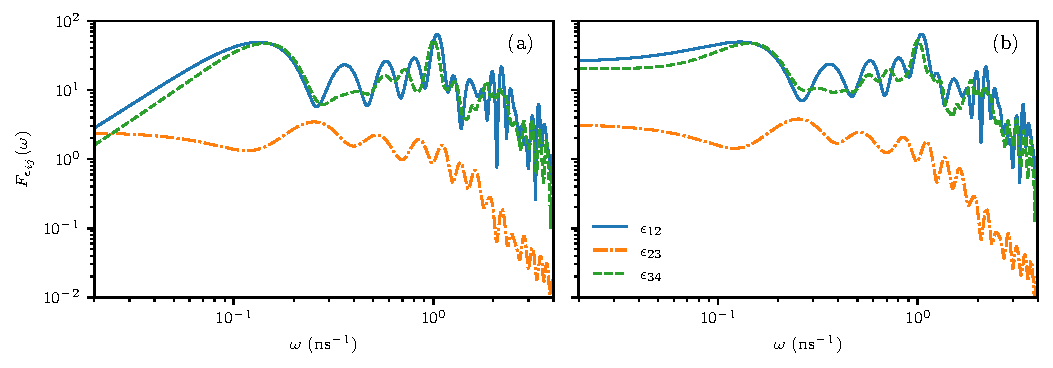
\includegraphics{img/pdf/filter_function-CNOT_unitary_v_complete}
    \caption{
        Filter functions of the voltage detunings $\epsilon_{ij}$ excluding (a) and including (b) the zero-padded identity matrix basis element $C_0^c\propto\text{diag}(1,1,1,1,0,0)$ for the computational subspace.
        Evidently, including $C_0^c$ removes the DCG character, namely that $F_{\epsilon_{ij}}(\omega)\rightarrow 0$ as $\omega\rightarrow 0$, of the gates but has little effect on the high-frequency behavior.
        As the pulse optimization minimizes, among other figures of merit, the infidelity of the final propagator mapped to the closest unitary on the computational subspace due to quasistatic and fast white noise, this indicates that excluding $C_0^c$ from the filter function corresponds to partially neglecting non-unitary components of the propagator on the computational subspace.
}
    \label{appfig:ff:filter_function:cnot}
\end{figure}

% ==================================================
%           QFT GATES SECTION
% ==================================================
\section{GRAPE-optimized gate set for QFT}\label{sec:app:ff:qft}
For completeness, in this appendix we give details on the GRAPE-optimized pulses for the gate set $\mathbb{G} = \lbrace\mr{X}_{i}(\flatfrac{\pi}{2}),\mr{Y}_{i}(\flatfrac{\pi}{2}),\mr{CR}_{ij}(\flatfrac{\pi}{2^3})\rbrace$ used in \cref{sec:ff:examples:qft} to simulate a \gls{qft} algorithm.
As mentioned in the main text, we consider a toy Rabi driving model with IQ single-qubit control and exchange to mediate inter-qubit coupling.
Cast in the language of quantum optimal control theory this translates to a vanishing drift (static) Hamiltonian, $H_\mr{d} =  0$, and a control Hamiltonian in the rotating frame given by
\begin{gather}
    \Hc(t) = \Hc\gth{0}(t)\otimes\eye + \eye\otimes\Hc\gth{1}(t) + \Hc\gth{01}(t), \\
    \Hc\gth{i}(t) = I_i(t)\px\gth{i} + Q_i(t)\py\gth{i},\qquad\Hc\gth{ij}(t) = J_{ij}(t)\pz\gth{i}\otimes\pz\gth{j},
\end{gather}
where $I_i(t)$ and $Q_i(t)$ are the in-phase and quadrature pulse envelopes and $\sigma_{x,y}\gth{i}$ are the Pauli matrices acting on the $i$-th and extended trivially to the other qubit.
As our goal is only of illustrative nature and not to provide a detailed gate optimization, we obtain the controls $\lbrace I_0(t), Q_0(t), I_1(t), Q_1(t), J_{12}(t)\rbrace$ for the gate set $\mathbb{G}$ using the GRAPE algorithm implemented in \qutip~\cite{Johansson2012} initialized with randomly distributed amplitudes.
The resulting pulses and the corresponding filter functions for the relevant noise operators are shown in \cref{appfig:ff:qft:gates}.

\begin{figure}
    \centering
    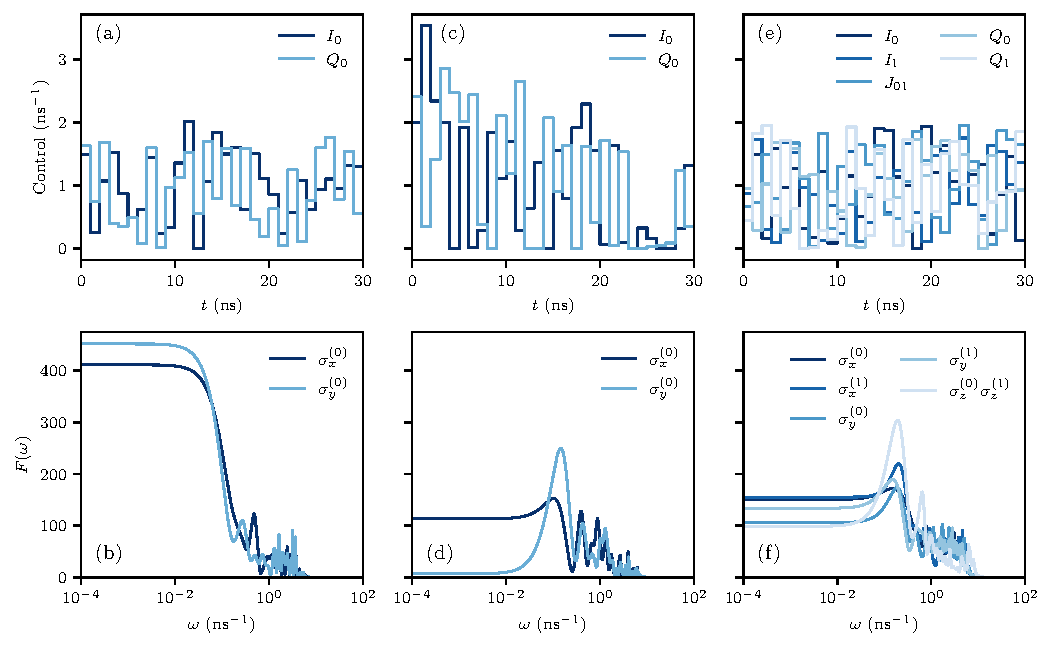
\includegraphics{img/pdf/qft_atomic_pulses}
    \caption{
        Control fields (top row) and corresponding filter functions (bottom row) of the GRAPE-optimized pulses in $\mathbb{G}$.
        (a),(b) $\text{X}_0(\flatfrac{\pi}{2})$; (c),(d) $\text{Y}_0(\flatfrac{\pi}{2})$; (e),(f) $\text{CR}_{01}(\flatfrac{\pi}{2^3})$.
        Note that the optimization is neither very sophisticated nor realistic as the algorithm only maximizes the systematic (coherent) fidelity $\mr{tr}\bigl(UQ\adjoint_\mr{targ}\bigr)/d$ and the randomly distributed initial control amplitudes are not subject to any constraints.
    }
    \label{appfig:ff:qft:gates}
\end{figure}

% ==================================================
%           CONVERGENCE SECTION
% ==================================================
\section{Convergence Bounds}\label{sec:app:ff:convergence}
In this appendix we give bounds for the convergence of the expansions employed in the main text for the case of purely auto-correlated noise, $S_{\alpha\beta}(\omega) = \delta_{\alpha\beta}S_{\alpha\beta}(\omega) =  S_\alpha(\omega)$, following the approach by~\citeauthor{Green2013}.
For Gaussian noise, our expansion is exact when including first and second order \acrfull{me} terms.
Hence, the convergence radius of the \gls{me} becomes infinite and the fidelity can be computed exactly by evaluating the matrix exponential \cref{eq:ff:cumulant}.
For non-Gaussian noise, the following considerations apply.
\subsection{Magnus Expansion}\label{sec:app:ff:convergence:magnus_expansion}
The \gls{me} of the error propagator \cref{eq:ff:magnus_expansion:1} converges if $\int_0^\tau\dd{t}\norm*{\Hnt(t)} < \pi$ with $\norm{A}^2 = \dotHS{A}{A} = \sum_{ij}\abs{A_{ij}}^2$ the Frobenius norm~\cite{Moan1999}.
We assume a time dependence of the noise operators of the form $\Ba(t) = s_\alpha(t)\Ba$.
By the Cauchy-Schwarz inequality we then have
\begin{equation}
    \begin{split}
        \bigl\lVert\Hnt(t)\bigr\rVert^2 &= \norm{\Hn(t)}^2 \\
                          &= \sum_{\alpha\beta} s_\alpha(t) s_{\beta}(t) b_\alpha(t) b_{\beta}(t)\dotHS{B_\alpha}{B_{\beta}} \\
                          &\leq\sum_{\alpha\beta} s_\alpha(t) s_{\beta}(t) b_\alpha(t) b_{\beta}(t)
                             \norm{B_\alpha}\norm{B_{\beta}} \\
                          &\leq\biggl[\sum_{\alpha}\sum_{g=1}^{G}\vartheta\gth{m}(t)
                             s_\alpha\gth{m}b_\alpha\gth{m}\norm{B_\alpha}\biggr]^2
    \end{split}
\end{equation}
where $b_{\alpha}\gth{m}$ is the maximum value that the noise assumes during the pulse, $\vartheta\gth{g}(t) = \theta(t - t_{g-1}) - \theta(t - t_g)$ is one during the $g$-th time interval and zero else, and where we approximated the time evolution as piecewise constant.
Then, in order to guarantee convergence of the \gls{me},
\begin{equation}
    \begin{split}
        \int_0^{\tau}\dd{t}\norm*{\Hnt(t)} &\leq\int_0^\tau\dd{t}\abs\bigg{\sum_{\alpha}\sum_{g=1}^{G}
                                              \vartheta\gth{m}(t) s_\alpha\gth{m} b_\alpha\gth{m}\norm{B_\alpha}} \\
                                           &= \sum_{\alpha} b_\alpha\gth{m}\norm{B_\alpha}\sum_{g=1}^{G}s_\alpha\gth{m}
                                              \int_{t_{g-1}}^{t_{g}}\dd{t} \\
                                           &= \sum_{\alpha} C_m\delta b_\alpha\norm{B_\alpha}\sum_{g=1}^{G}
                                              s_\alpha\gth{m}\Delta t_g \\
                                           &\eqqcolon N
    \end{split}
\end{equation}
where we have expressed the in principle unknown maximum noise amplitude $b_\alpha\gth{m}$ in terms of the root mean square value $\delta b_\alpha$.
That is, $b_\alpha\gth{m} = C_m \expval*{b_\alpha(0)^2}^{1/2} =  C_m \delta b_\alpha$ for a sufficiently large value $C_m$.
Finally, realizing that $\delta b_\alpha^2 = \int\frac{\dd{\omega}}{2\pi} S_\alpha(\omega)$ and by the triangle inequality,
\begin{equation}
    \begin{split}
        N &= C_m\sum_{\alpha}\norm{B_\alpha}\biggl[\int_{-\infty}^\infty\frac{\mathrm{d}\omega}{2\pi} S_\alpha(\omega)\biggr]^{1/2}
            \sum_{g=1}^{G} s_\alpha\gth{m}\Delta t_g \\
          &\leq C_m\biggl[\sum_{\alpha}\norm{B_\alpha}^2\int_{-\infty}^\infty\frac{\mathrm{d}\omega}{2\pi} S_\alpha(\omega)
            \biggl(\sum_{g=1}^{G} s_\alpha\gth{m}\Delta t_g\biggr)^2\biggr]^{1/2} \\
          &\eqqcolon C_m\xi \\
          &\overset{!}{<} \pi
    \end{split}
\end{equation}
where we have introduced the parameter $\xi$.
Thus, the expansion converges if $\xi < \flatfrac{\pi}{C_m}$.
However, we note that in practice the rms noise amplitude $\delta b_\alpha$ will often be infinite, limiting the usefulness of this bound for certain noise spectra.
\subsection{Infidelity}\label{sec:app:ff:convergence:infidelity}
Again assuming a time dependence $\Ba(t) = s_\alpha(t)\Ba$ as well as piecewise constant control, we note that for the infidelity we have (\cf \cref{eq:ff:fidelity:ent})
\begin{equation}
    \begin{split}
        \abs{\tr(\decayamps)} &= \abs\Bigg{\sum_{\alpha}\int_0^\tau\dd{t_2}\int_0^\tau\dd{t_1}
                                 \expval{b_\alpha(t_1)b_\alpha(t_2)}\sum_{k}\ctrlmat_{\alpha k}(t_1)\ctrlmat_{\alpha k}(t_2)} \\
                              &\leq\abs\Bigg{\sum_{\alpha}\int_0^\tau\dd{t_2}\int_0^\tau\dd{t_1}
                                 \expval{b_\alpha(t_1)b_\alpha(t_2)}\sum_{g,g'=1}^{G}\vartheta\gth{m}(t_1)\vartheta^{(g')}(t_2)
                                 s_\alpha\gth{m} s_\alpha^{(g')} \norm{B_\alpha}^2} \\
                              &\leq\sum_{\alpha}\norm{B_\alpha}^2
                                 \underbrace{\expval{b_\alpha^2(0)}}_{\int\frac{\dd{\omega}}{2\pi}S_\alpha(\omega)}
                                 \sum_{g,g'=1}^{G} s_\alpha\gth{m} s_\alpha^{(g')}
                                 \abs\Bigg{\int_{t_{g'-1}}^{t_{g'}}\dd{t_2}\int_{t_{g-1}}^{t_g}\dd{t_1}
                                 \underbrace{\overline{\expval{b_\alpha(t_1)b_\alpha(t_2)}}}_{\abs{\placeholder}\leq 1}} \\
                              &\leq\sum_{\alpha}\left[\norm{B_\alpha}^2
                                 \int_{-\infty}^\infty\frac{\mathrm{d}\omega}{2\pi}S_\alpha(\omega)
                                 \biggl(\sum_{g=1}^{G}s_\alpha\gth{m}\Delta t_g\biggr)^2\right] \\
                              &= \xi^2,
    \end{split}
\end{equation}
where, going from the second to the third line, we have factored out the total power of noise source $\alpha$ from the cross-correlation function, $\expval{b_\alpha(t_1) b_\alpha(t_2)} = \expval{b_\alpha^2(0)}\bigl\lvert\overline{\expval{b_\alpha(t_1)b_\alpha(t_2)}}\bigr\rvert$.
Thus, the first order infidelity \cref{eq:ff:fidelity:ent} is upper bounded by $\flatfrac{\xi^2}{d}$, the same parameter also bounding the convergence of the \gls{me}, and higher orders can be neglected if $\xi^2\ll 1$.

Note that similar arguments can be made for the higher orders of the \gls{me}~\cite{Green2013}.
In particular, the $n$-th order \gls{me} term containing $n$-point correlation functions of the noise is of order $\order{\xi^n}$ as stated in the main text.

\section{Second-order concatenation}\label{sec:app:ff:concatenation}
In this appendix, I lay out how the second-order filter functions of atomic pulse segments can be re-used to compute the filter function of the concatenated sequence.
While it is not possible, due to the nested time integral\todo{refeq}, to perform the calculation entirely without concern for the internal structure of the individual segments, it is also not necessary to compute everything from scratch.
